\documentclass[journal,12pt,twocolumn]{IEEEtran}

\usepackage{setspace}
\usepackage{gensymb}

\singlespacing


\usepackage[cmex10]{amsmath}

\usepackage{amsthm}

\usepackage{mathrsfs}
\usepackage{txfonts}
\usepackage{stfloats}
\usepackage{bm}
\usepackage{cite}
\usepackage{cases}
\usepackage{subfig}

\usepackage{longtable}
\usepackage{multirow}

\usepackage{enumitem}
\usepackage{mathtools}
\usepackage{steinmetz}
\usepackage{tikz}
\usepackage{circuitikz}
\usepackage{verbatim}
\usepackage{tfrupee}
\usepackage[breaklinks=true]{hyperref}

\usepackage{tkz-euclide}

\usetikzlibrary{calc,math}
\usepackage{listings}
    \usepackage{color}                                            %%
    \usepackage{array}                                            %%
    \usepackage{longtable}                                        %%
    \usepackage{calc}                                             %%
    \usepackage{multirow}                                         %%
    \usepackage{hhline}                                           %%
    \usepackage{ifthen}                                           %%
    \usepackage{lscape}     
\usepackage{multicol}
\usepackage{chngcntr}

\DeclareMathOperator*{\Res}{Res}

\renewcommand\thesection{\arabic{section}}
\renewcommand\thesubsection{\thesection.\arabic{subsection}}
\renewcommand\thesubsubsection{\thesubsection.\arabic{subsubsection}}

\renewcommand\thesectiondis{\arabic{section}}
\renewcommand\thesubsectiondis{\thesectiondis.\arabic{subsection}}
\renewcommand\thesubsubsectiondis{\thesubsectiondis.\arabic{subsubsection}}


\hyphenation{op-tical net-works semi-conduc-tor}
\def\inputGnumericTable{}                                 %%

\lstset{
%language=C,
frame=single, 
breaklines=true,
columns=fullflexible
}
\begin{document}


\newtheorem{theorem}{Theorem}[section]
\newtheorem{problem}{Problem}
\newtheorem{proposition}{Proposition}[section]
\newtheorem{lemma}{Lemma}[section]
\newtheorem{corollary}[theorem]{Corollary}
\newtheorem{example}{Example}[section]
\newtheorem{definition}[problem]{Definition}

\newcommand{\BEQA}{\begin{eqnarray}}
\newcommand{\EEQA}{\end{eqnarray}}
\newcommand{\define}{\stackrel{\triangle}{=}}
\bibliographystyle{IEEEtran}
\providecommand{\mbf}{\mathbf}
\providecommand{\pr}[1]{\ensuremath{\Pr\left(#1\right)}}
\providecommand{\qfunc}[1]{\ensuremath{Q\left(#1\right)}}
\providecommand{\sbrak}[1]{\ensuremath{{}\left[#1\right]}}
\providecommand{\lsbrak}[1]{\ensuremath{{}\left[#1\right.}}
\providecommand{\rsbrak}[1]{\ensuremath{{}\left.#1\right]}}
\providecommand{\brak}[1]{\ensuremath{\left(#1\right)}}
\providecommand{\lbrak}[1]{\ensuremath{\left(#1\right.}}
\providecommand{\rbrak}[1]{\ensuremath{\left.#1\right)}}
\providecommand{\cbrak}[1]{\ensuremath{\left\{#1\right\}}}
\providecommand{\lcbrak}[1]{\ensuremath{\left\{#1\right.}}
\providecommand{\rcbrak}[1]{\ensuremath{\left.#1\right\}}}
\theoremstyle{remark}
\newtheorem{rem}{Remark}
\newcommand{\sgn}{\mathop{\mathrm{sgn}}}
\providecommand{\abs}[1]{\left\vert#1\right\vert}
\providecommand{\res}[1]{\Res\displaylimits_{#1}} 
\providecommand{\norm}[1]{\left\lVert#1\right\rVert}
%\providecommand{\norm}[1]{\lVert#1\rVert}
\providecommand{\mtx}[1]{\mathbf{#1}}
\providecommand{\mean}[1]{E\left[ #1 \right]}
\providecommand{\fourier}{\overset{\mathcal{F}}{ \rightleftharpoons}}
%\providecommand{\hilbert}{\overset{\mathcal{H}}{ \rightleftharpoons}}
\providecommand{\system}{\overset{\mathcal{H}}{ \longleftrightarrow}}
	%\newcommand{\solution}[2]{\textbf{Solution:}{#1}}
\newcommand{\solution}{\noindent \textbf{Solution: }}
\newcommand{\cosec}{\,\text{cosec}\,}
\providecommand{\dec}[2]{\ensuremath{\overset{#1}{\underset{#2}{\gtrless}}}}
\newcommand{\myvec}[1]{\ensuremath{\begin{pmatrix}#1\end{pmatrix}}}
\newcommand{\mydet}[1]{\ensuremath{\begin{vmatrix}#1\end{vmatrix}}}
\numberwithin{equation}{subsection}
\makeatletter
\@addtoreset{figure}{problem}
\makeatother
\let\StandardTheFigure\thefigure
\let\vec\mathbf
\renewcommand{\thefigure}{\theproblem}
\def\putbox#1#2#3{\makebox[0in][l]{\makebox[#1][l]{}\raisebox{\baselineskip}[0in][0in]{\raisebox{#2}[0in][0in]{#3}}}}
     \def\rightbox#1{\makebox[0in][r]{#1}}
     \def\centbox#1{\makebox[0in]{#1}}
     \def\topbox#1{\raisebox{-\baselineskip}[0in][0in]{#1}}
     \def\midbox#1{\raisebox{-0.5\baselineskip}[0in][0in]{#1}}
\vspace{3cm}
\title{Assignment 6}
\author{Gaydhane Vaibhav Digraj \\ Roll No. AI20MTECH11002}
\maketitle
\newpage
\bigskip
\renewcommand{\thefigure}{\theenumi}
\renewcommand{\thetable}{\theenumi}
\begin{abstract}
This document finds the equation of lines which are tangent to the curve. 
\end{abstract}
%
Download latex-tikz codes from 
%
\begin{lstlisting}
https://github.com/Vaibhav11002/EE5609/tree/master/Assignment_6
\end{lstlisting}
%
\section{Problem}
Find the equation of all lines having slope $-2$ which are tangents to the curve $\frac{1}{x-3}$, $x\ne3$. 

\section{Solution}
Given the curve, 
\begin{align}
    y = \frac{1}{x-3} \label{eq:1}\\ 
    \implies xy-3y-1 = 0 \label{eq:2}
\end{align}
From \eqref{eq:2} we get,  
\begin{align}
    \vec{V} = \frac{1}{2}\myvec{0 & 1 \\ 1 & 0}, \vec{u} = \frac{-3}{2}\myvec{0 \\ 1}, f=-1
\end{align}
Now, 
\begin{align}
    \because \mydet{V} = \mydet{0&\frac{1}{2}\\\frac{1}{2}&0} = \frac{-1}{2}<0
\end{align}

\eqref{eq:1} is equation of hyperbola. Now, 
\begin{align}
    \mydet{\lambda\vec{I}-\vec{V}} = \mydet{\lambda & \frac{-1}{2}\\\frac{-1}{2} & \lambda}=0 \\
    \implies \lambda^2-\frac{1}{4} =0
\end{align}
Thus the eigen values are, 
\begin{align}
    \lambda_1 = \frac{1}{2}, \lambda_2 = \frac{-1}{2}
\end{align}
The eigen vector \vec{p} is given by,
\begin{align}
    (\lambda\vec{I}-\vec{V})\vec{p}=0
\end{align}
For $\lambda_1 = \frac{1}{2}$,

\begin{align}
    (\lambda_1 \vec{I}-\vec{V}) = \myvec{\frac{1}{2}&\frac{1}{2}\\\frac{1}{2}&\frac{1}{2}}
    \xleftrightarrow[R_1\xleftarrow{}2R_1]{R_2\xleftarrow{}R_2+R_1}
    \myvec{1&-1\\0&0} \\
    \implies \vec{p_1} = \frac{1}{\sqrt{2}}\myvec{1\\1}
\end{align}
Similarly for $\lambda_2$,
\begin{align}
    (\lambda_2 \vec{I}-\vec{V}) = \myvec{\frac{-1}{2}&\frac{-1}{2}\\\frac{-1}{2}&\frac{-1}{2}}
    \xleftrightarrow[R_1\xleftarrow{}2R_1]{R_2\xleftarrow{}R_-R_1}
    \myvec{1&1\\0&0} \\
    \implies \vec{p_2} = \frac{1}{\sqrt{2}}\myvec{-1\\1}
\end{align}
Now, 
\begin{align}
    \vec{P} = \myvec{\vec{p_1}&\vec{p_2}} = \frac{1}{\sqrt{2}}\myvec{1&-1\\1&1} \\
    \vec{D} = \myvec{\frac{1}{2}&0\\0&\frac{-1}{2}} \\
    \vec{u}^T\vec{V}^{-1}\vec{u}-f=1
\end{align}
\because $\vec{u}^T\vec{V}^{-1}\vec{u}-f=1>0$, there is no need to swap the axes. The hyperbola parameters are, 
\begin{align}
    \vec{c} = -\vec{V}^{-1}\vec{u} = 3\myvec{1\\0} \\
    \sqrt{\frac{\vec{u}^T\vec{V}^{-1}\vec{u}-f}{\lambda_1}}=\sqrt{2} \\
    \sqrt{\frac{f-\vec{u}^T\vec{V}^{-1}\vec{u}}{\lambda_1}}=\sqrt{2}
\end{align}
with the standard hyperbola becoming, 
\begin{align}
    \frac{x^2}{2}-\frac{y^2}{2}=1
\end{align}
The direction and normal vectors of the tangent with slope $-2$ are given as,
\begin{align}
    \vec{m}=\myvec{1\\-2}, \vec{n}=\myvec{2\\1}
\end{align}
Now considering the equations to find the point of contact, 
\begin{align}
    \vec{q}=\vec{V}^{-1}(k\vec{n}-\vec{u}) \\
    k = \pm \sqrt{\frac{\vec{u}^T\vec{V}^{-1}\vec{u}-f}{\vec{n}^T\vec{V}^{-1}\vec{n}}}
\end{align}
Thus, 
\begin{align}
    \vec{n}^T\vec{V}^{-1}\vec{n}=8 \\
    k= \pm \frac{1}{2\sqrt{2}} \\
    \vec{q_1} = \myvec{\frac{1+3\sqrt{2}}{\sqrt{2}} \\ \sqrt{2}} \\
    \vec{q_2} = \myvec{\frac{-1+3\sqrt{2}}{\sqrt{2}} \\ -\sqrt{2}}
\end{align}
The desired tangents are, 
\begin{align}
    \myvec{2&1} \cbrak{\vec{x}-\myvec{\frac{1+3\sqrt{2}}{\sqrt{2}} \\ \sqrt{2}}} = 0 \\ 
    \implies \myvec{2&1}\vec{x} = 6+2\sqrt{2} \label{tangent_1} \\
    \myvec{2&1} \cbrak{\vec{x}-\myvec{\frac{-1+3\sqrt{2}}{\sqrt{2}} \\ -\sqrt{2}}} = 0 \\
    \implies \myvec{2&1}\vec{x} = 6-2\sqrt{2}  \label{tangent_2}
\end{align}

Below figure corresponds to the tangents on the hyperbola,  represented by \eqref{tangent_1} and \eqref{tangent_2} each having slope of $-2$. 
\renewcommand{\thefigure}{\arabic{figure}}
\begin{figure}[h!]
	\centering
	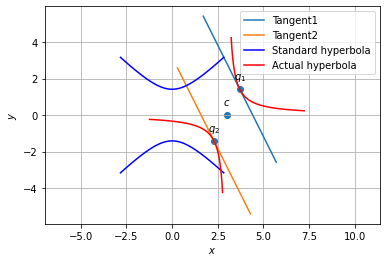
\includegraphics[width=\columnwidth]{assignment_6.png}
	\caption{Tangents to the hyperbola}
	\label{fig_1}
\end{figure}



\end{document}